\documentclass[10pt,a4paper]{beamer}
\usetheme{Copenhagen}
\usecolortheme{beaver}
\useinnertheme{rounded}
\usepackage[latin1]{inputenc}
\usepackage{amsmath}
\usepackage{amsfonts}
\usepackage{amssymb}
\usepackage{algorithmic}
\usepackage{wrapfig}
\usepackage{listings}
\usepackage{adjustbox}
\usepackage{url}
\usepackage{verbatim}
\usepackage{tikz}
\usetikzlibrary{calc, positioning,fit,intersections}
\usetikzlibrary{graphs}

\logo{
\includegraphics{figures/logo20.jpg}}
\setbeamertemplate{blocks}[rounded][shadow=true]
\author{Sergio Hern\'andez, Jos\'e Vald\'es and Matias Valdenegro}
\institute
{
  \inst{1}%
    Laboratorio de Procesamiento de Informaci\'on Geoespacial.\\
	Universidad Cat\'olica del Maule. Chile\\ 
	\tt{shernandez@ucm.cl}
	\and
	\inst{2}%
	Centro de Innovaci\'on en Ingenier\'ia Aplicada.\\
	Universidad Cat\'olica del Maule. Chile.\\
	\and 
    \inst{3}%
	German Research Center for Artificial Intelligence\\
	Robotics Innovation Center. Germany.\\ 
}
\date{INGELECTRA XXVIII}
\title[A comparison of SG-MCMC using Multi-Core and GPU Architectures]{A Comparison of Stochastic Gradient MCMC using Multi-Core and GPU Architectures}

\begin{document}

\begin{frame}
\titlepage
\end{frame}

\begin{frame}\frametitle{Introduction}
\begin{columns}
	\column{0.5\textwidth}
	\begin{itemize}
		\item Deep learning models are traditionally used in big data scenarios.
		\item Stochastic Gradient Descent (SGD) is an optimization technique traditionally used for out-of-core training deep learning.
		\item Bayesian inference techniques can be used to capture the uncertainty of the model but it comes with a high computational cost. 
	\end{itemize}
	\column{0.5\textwidth}
	\begin{figure}
			\centering
			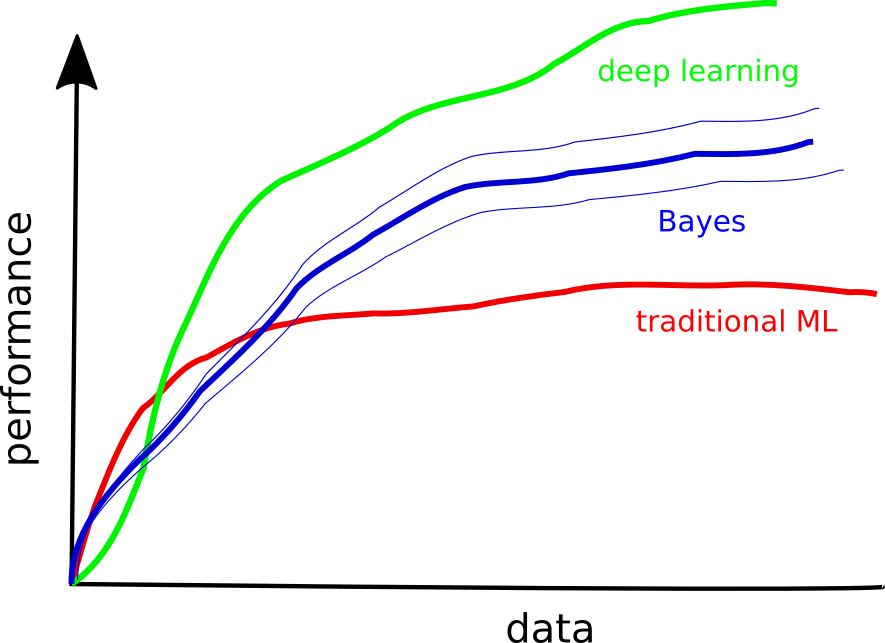
\includegraphics[width=1.2\linewidth]{figures/schematic_data}
			\label{fig:schematicdata}
	\end{figure}

	
\end{columns}
\end{frame}

\begin{frame}\frametitle{Stochastic Gradient MCMC}
\begin{itemize}
	\item Let $\mathbf{D}=\{\mathbf{d_1},\ldots,\mathbf{d_N}\}$ represent a typical dataset used for classification problems, as a set of tuples $\mathbf{d}=(\mathbf x,y)$ that contains features $\mathbf x \in \mathbb R^D$ and labels $y=\{1,\ldots,K\}$. 
	\pause
	\item  SGD iterates  over mini-batches of size $B \ll N$ and computes a point estimate $\theta^\ast$. 
	\pause
	\item In the Bayesian framework, the unknown parameter $\theta$ is considered as a random variable.
\end{itemize}
\pause
\resizebox{11cm}{!}{
	\begin{columns}[T]
		\column{0.5\textwidth}
		\begin{alertblock}{SGD (Robbins \& Monro, 1951)}
			$\theta^\ast = \operatorname{argmax} p(\mathbf{D} \vert \theta)$
		\end{alertblock} 
		\begin{block}{SGLD (Welling \& Teh, 2013)}
			$p(\theta \vert \mathbf{D}) = \frac{p(\mathbf{D} \vert \theta)p(\theta)}{\int p(\mathbf{D} \vert \theta)p(\theta) d\theta}$
		\end{block}
		\column{0.5\textwidth}
		\begin{alertblock}{SGD update}
			$\theta_{t+1}=\theta_{t}+\Big(\epsilon_t \sum_i^B \nabla \operatorname{log} p(\mathbf{d_i} \vert \theta_{t})\Big)$
		\end{alertblock}
		\begin{block}{SGLD update}
			$\theta_{t+1}=\theta_{t}+\frac{\epsilon_t}{2}\Big(\nabla\operatorname{log}p(\theta_{t})+\frac{N}{B} \sum_i^B \nabla \operatorname{log} p(\mathbf{d_i} \vert \theta_{t})\Big) + \eta_t$
		\end{block}
	\end{columns}
}
\end{frame}

\begin{frame}\frametitle{CPU/GPU SG-MCMC}
	\begin{columns}[T]
	\column{0.5\textwidth}
	\begin{figure}
			
\includegraphics[width=\textwidth]{figures/gpu_architechture}
			\caption{GPU implementation.}
			\label{fig:gpuarchitechture}
			
		\end{figure}
	\column{0.5\textwidth}
	\begin{figure}
			
\includegraphics[width=\textwidth]{figures/cpu_architechture}
			\caption{CPU implementation.}
			\label{fig:cpuarchitechture}
		\end{figure}
	\end{columns}
\end{frame}


\begin{frame}\frametitle{Experimental results}

\begin{columns}
	\column{0.5\textwidth}
	\begin{itemize}
		\item Serial versions of the SGD and SGLD algorithms are tested on CPU and compared with parallel
		implementations on GPU.
		\item All experiments are run on a server with an Intel Xeon E5-2620 CPU
		with 12 cores using a single fully connected softmax layer (which is widely used in transfer learning).
		\item The server is also equipped with an NVIDIA TITAN GPU and both implementations were developed
		using Python 3.4.9.
	\end{itemize}
	\column{0.5\textwidth}
	\begin{figure}
		\centering
		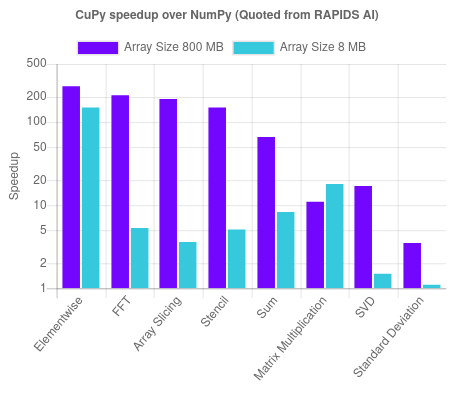
\includegraphics[width=\linewidth]{figures/cupy_numpy}
		\caption{\scriptsize{\url{https://medium.com/rapids-ai/single-gpu-cupy-speedups-ea99cbbb0cbb}}}
	\end{figure}
	
\end{columns}
\end{frame}

\begin{frame}\frametitle{Synthetic Data (SGD)}
The number of classes was set to $K=3$, the number of epochs was set to $E=2 \times 10^4$ and the size of the mini-batches was set to $B=50$ for all examples.
\begin{table}[h]
	\centering
	\begin{tabular}{|c|c|c|c|c|c|c|}
		\hline 
		D & N & CPU Time [s] & GPU Time [s]  & Speed-Up\\ 
		\hline 
		10 &	1000&	11.98&	124.85& 10.42\\
		10&	10000&	119.90&	1245.98& 10.39\\
		10&	50000&	594.71&	6186.05& 10.40\\
		10&	100000&	1195.62&	12261.716& 10.25\\
		\hline
		50&	1000&	13.67&	123.13& 9.00\\
		50&	10000&	135.96&	1230.19& 9.04\\
		50&	50000&	689.89&	6137.79& 8.89\\
		50&	100000&	1487.26&	12240.06& 8.22\\
		\hline
		100&	1000&	15.71&	123.53& 7.86\\
		100	&10000&	156.94&	1231.121& 7.84\\
		100&	50000&	806.78&	6176.91& 7.65\\
		100&	100000&	1770.83&	12394.13& 6.99\\
		\hline 
	\end{tabular}
	\caption{Run time comparison of CPU and GPU implementations of SGD for a softmax regression problem}
	\label{tab:sgd} 
\end{table}
\end{frame}

\begin{frame}\frametitle{Synthetic Data (SGLD)}
\begin{table}[h]
	\centering
	\begin{tabular}{|c|c|c|c|c|c|c|}
		\hline 
		D & N & CPU Time [s] & GPU Time [s]  & Speed-Up\\ 
		\hline 		
		10	& 1000& 	24.75& 294.04  & 11.87\\
		10	& 10000& 	245.22& 2946.67	& 12.01\\
		10	& 50000& 	1186.81& 14518.66 & 12.23\\
		10	& 100000	& 2380.18& 29010.43& 12.18\\
		\hline
		50	& 1000	& 25.70& 288.02	& 11.48\\
		50	& 10000	& 246.64& 2885.16& 11.69\\
		50	& 50000	& 1230.02& 14467.73	& 11.76\\
		50 & 	100000	& 2496.15& 28930.81	& 11.59\\
		\hline
		100	& 1000	& 30.95& 288.21& 9.31\\
		100	& 10000	& 279.28& 2903.20& 10.39\\
		100	& 50000	& 1450.57& 14531.93& 10.01\\
		100	& 100000& 	2796.20& 29117.73& 10.41\\
		
		\hline 
	\end{tabular}
	\caption{Run time comparison of CPU ans GPU implementations of SGLD for a softmax regression problem}
	\label{tab:sgld} 
\end{table}
\end{frame}

\begin{frame}\frametitle{Bayesian Transfer Learning}
\begin{itemize}
	\item The Plant Village dataset contains $54306$ images with combinations of $14$ crops and $26$ diseases, leaving a total number of $K=38$ classes.
	\item  The VGG16 deep neural network with weights trained on the Imagenet dataset is used to extract features with dimensionality $25088$ from the plants diseases dataset. 
	\item The original class distribution is unbalanced, therefore random over-sampling is used to achieve a uniform class distribution, leaving a total number os $N=203500$ training samples and $5700$ test samples.
	\end{itemize}


\begin{figure}
	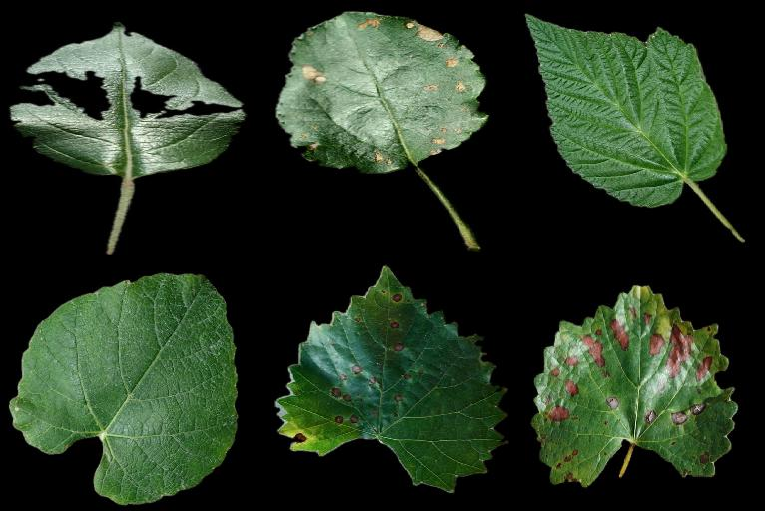
\includegraphics[width=\hsize]{figures/plant_village_subset}
	\caption{Leaf images from healthy and infected plants from the Plant Village dataset}
	\label{fig:plantvillagesubset}
\end{figure}
\end{frame}

\begin{frame}\frametitle{Bayesian Transfer Learning}
	\begin{columns}[T]
	\column{0.33\textwidth}
	\begin{figure}
		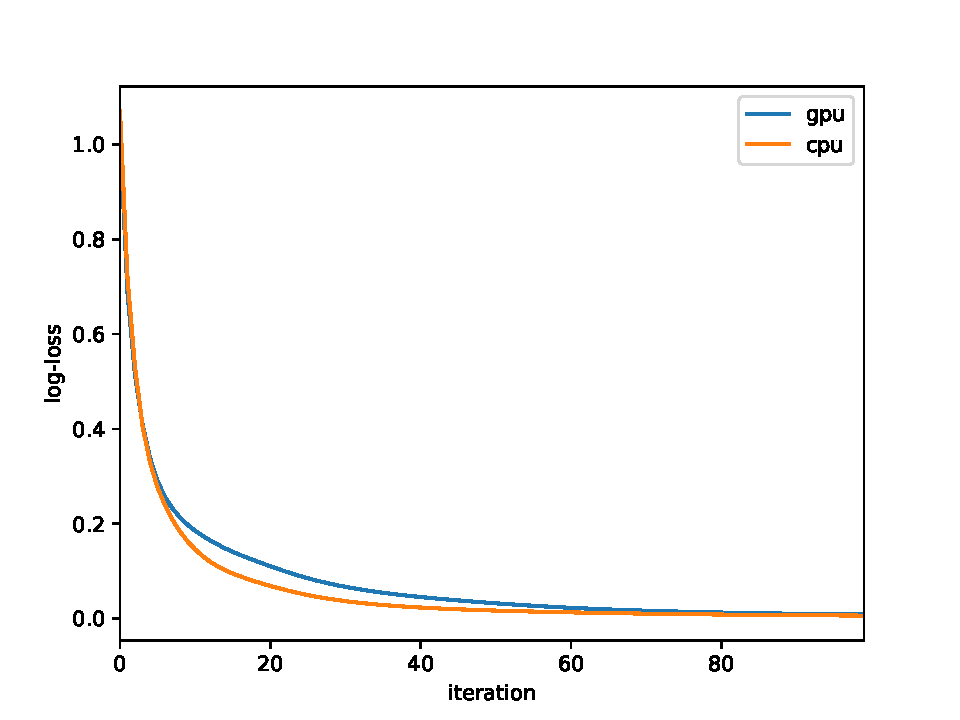
\includegraphics[width=\textwidth,height=3cm]{results/sgd_losloss}
	\end{figure}
	\column{0.33\textwidth}
	\begin{figure}
		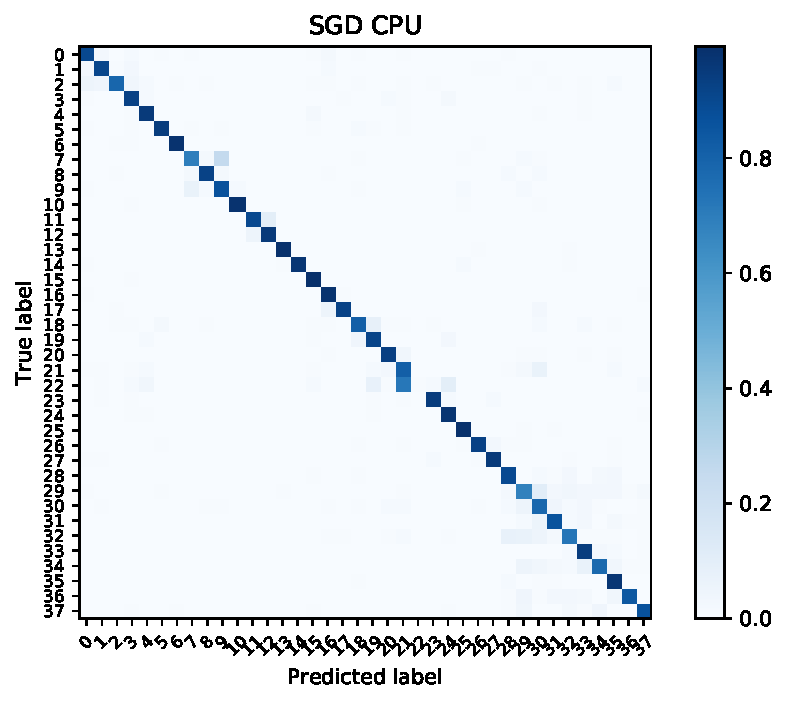
\includegraphics[width=\textwidth]{results/plants_confusion_matrix_sgd_cpu}
		\label{fig:sgd_cpu_performance}
	\end{figure}
	\column{0.33\textwidth}
	\begin{figure}
		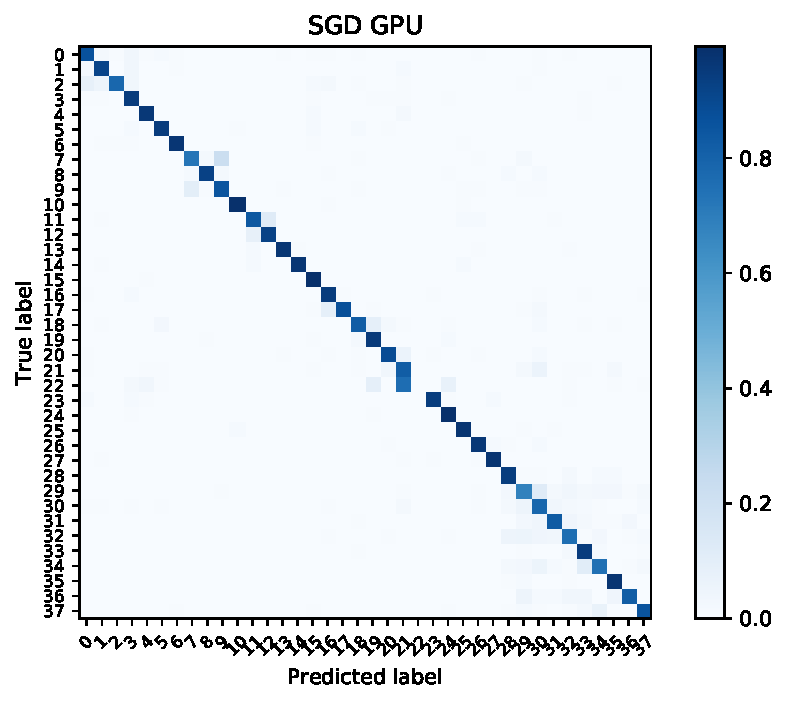
\includegraphics[width=\textwidth]{results/plants_confusion_matrix_sgd_gpu}
		\label{fig:sgd_gpu_performance}
	\end{figure}
\end{columns}
	\begin{columns}[T]
	\column{0.3\textwidth}
	\begin{figure}
		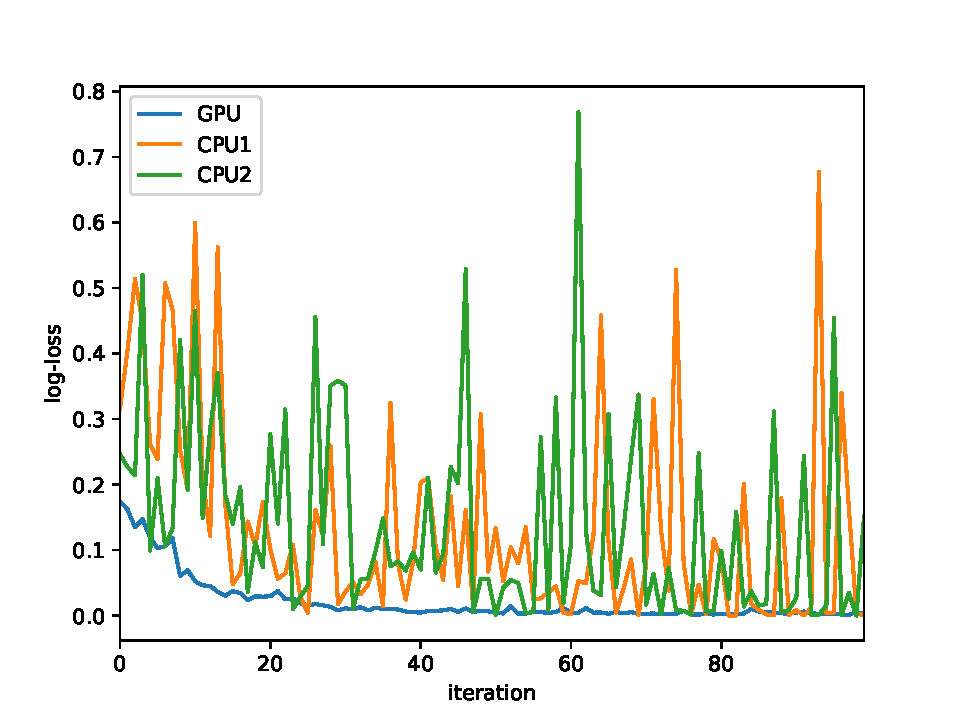
\includegraphics[width=\textwidth,height=3cm]{results/sgld_losloss}
	\end{figure}
	\column{0.3\textwidth}
	\begin{figure}
		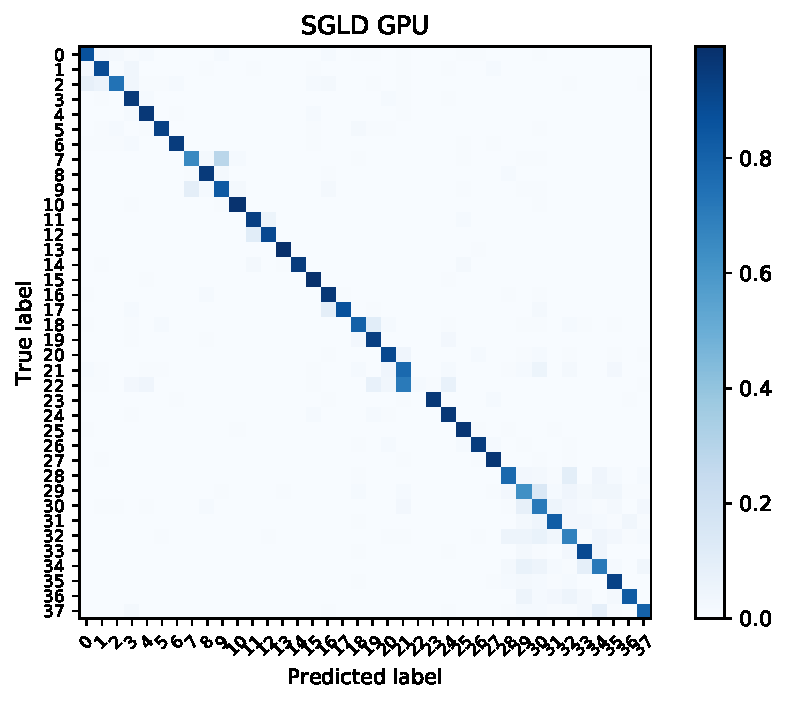
\includegraphics[width=\textwidth]{results/plants_confusion_matrix_sgld_gpu}
		\label{fig:sgld_cpu_performance}
	\end{figure}
	\column{0.3\textwidth}
	\begin{figure}
		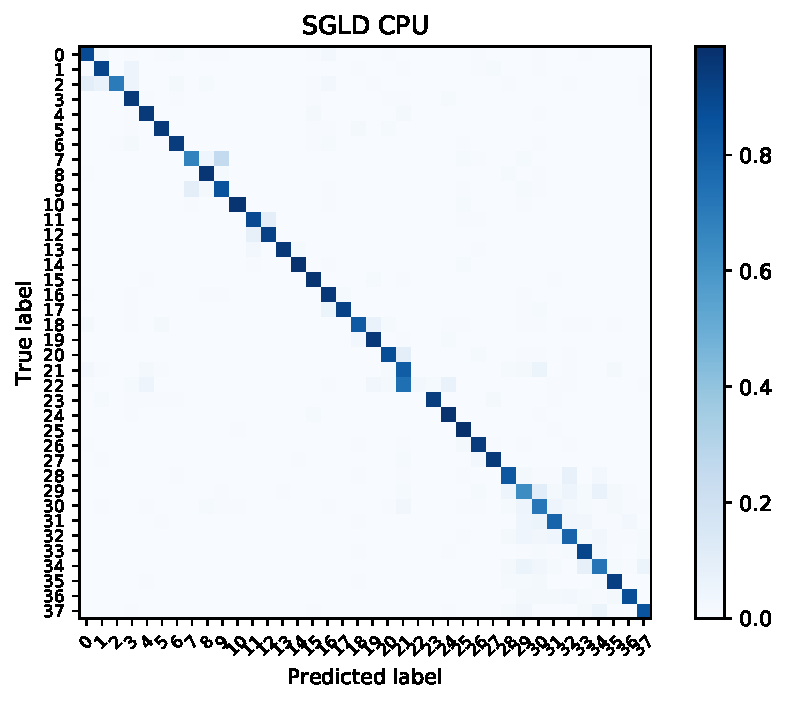
\includegraphics[width=\textwidth]{results/plants_confusion_matrix_sgld_cpu}
		\label{fig:sgld_gpu_performance}
	\end{figure}
\end{columns}
\end{frame}


\begin{frame}\frametitle{Conclusions}
\begin{itemize}
	\item In this work, a novel comparison between multi-core CPU and GPU architectures for SGLD is performed. 
	\item  The speedups achieved with synthetic data are not compatible with other real data sets such as transfer learning data sets, which is mainly due to the size of the data batches and the model parameters. 
	\item Future work will consider hybrid approaches based on multi-core CPU and multi-GPU that could also be beneficial in real life scenarios. 
\end{itemize}
\end{frame}
\end{document}